\documentclass[11pt]{article}

\usepackage[margin=1in]{geometry}
\usepackage{fontspec}
\setmainfont{Times New Roman}
\usepackage{graphicx}
\usepackage{booktabs}
\usepackage{array}
\usepackage{xcolor}
\usepackage{hyperref}
\usepackage{caption}
\usepackage{float}
\usepackage{amsmath}
\usepackage{enumitem}
\usepackage{titlesec}
\usepackage{fancyhdr}
\usepackage{longtable}
\usepackage{multirow}
\usepackage{parskip}
\usepackage{microtype}

\emergencystretch=3em
\sloppy

\hypersetup{colorlinks=true, linkcolor=black, citecolor=black, urlcolor=blue, pdftitle={Assignment 04 - Comparing CNN and MLP Implementations}}

\pagestyle{fancy}
\fancyhf{}
\fancyfoot[C]{\thepage}
\renewcommand{\headrulewidth}{0pt}
\renewcommand{\footrulewidth}{0pt}

\titleformat{\section}{\normalfont\Large\bfseries}{\thesection}{1em}{}
\titleformat{\subsection}{\normalfont\large\bfseries}{\thesubsection}{1em}{}
\titleformat{\subsubsection}{\normalfont\normalsize\bfseries}{\thesubsubsection}{1em}{}

\newcommand{\model}[1]{\textbf{#1}}
\newcommand{\code}[1]{\texttt{#1}}
\newcommand{\impl}[1]{\textbf{#1}}

\begin{document}

% ---------------------------------------------------------------------
% Cover page
% ---------------------------------------------------------------------
\begin{titlepage}
\centering
\vspace*{2cm}
{\Large INTELLIGENT SYSTEM DEVELOPMENT}\\[0.3cm]
{\Large ASSIGNMENT 04}\\[0.5cm]
{\huge \bfseries Comparing CNN and MLP Implementations: Scratch vs. Keras vs. PyTorch}\\[2cm]

\begin{tabular}{ll}
Authors: & Bùi Nguyên Hoàng Việt (B23DCDT285) \\
         & Lưu Anh Dũng (B23DCDK036) \\
         & Nguyễn Văn Trường (B23DCCE095) \\[0.5cm]
Class: & E23CNPM02 \\[0.5cm]
Course: & Intelligent System Development \\[0.5cm]
Lecturer: & Assoc. Prof. Dinh Que Tran, Ph.D. \\[0.5cm]
Semester: & I.2026 \\
\end{tabular}

\vfill
{\large Three applications, one MLP and two CNNs, each built and trained three
separate times, from scratch in NumPy, in TensorFlow/Keras, and in PyTorch, to
compare abstraction level rather than to compare models against each other.}
\end{titlepage}

\tableofcontents
\newpage

% ---------------------------------------------------------------------
\section{Executive Summary}
% ---------------------------------------------------------------------

This report builds three intelligent systems, diabetes risk screening (tabular,
binary classification), Fashion-MNIST clothing recognition (grayscale image,
10-class classification), and CIFAR-10 object recognition (RGB image, 10-class
classification), each with a single architecture implemented three separate
times: from scratch in NumPy with no deep learning framework, in
TensorFlow/Keras, and in PyTorch. The point of the assignment is not to find
the best of nine trained models. It is to test Lecture 04's central claim
directly: that the same learning problem, expressed as the same architecture,
should produce close to the same result regardless of which of the three
abstraction levels builds it, and that what actually differs between the three
is code visibility, developer convenience, and training speed, not the
underlying mathematics.

Table \ref{tab:exec-summary} summarizes the three applications and which
implementation won by test accuracy, the assignment's primary comparison
metric.

\begin{table}[H]
\centering
\caption{Executive summary across the three applications}
\label{tab:exec-summary}
\small
\begin{tabular}{@{}p{2.2cm}p{2.4cm}p{2.6cm}p{2.9cm}p{2.6cm}@{}}
\toprule
Application & Data type & Task & Architecture & Winning implementation \\
\midrule
Diabetes & tabular & binary classification & MLP ($50 \to 32 \to 16 \to 1$) & PyTorch (0.782) \\
Fashion-MNIST & image, $28\times28\times1$ & 10-class classification & CNN (421,642 params) & Scratch (0.897) \\
CIFAR-10 & image, $32\times32\times3$ & 10-class classification & CNN (545,098 params) & Keras (0.610) \\
\bottomrule
\end{tabular}
\end{table}

Two results stand out ahead of the detailed sections below. First, the
parameter count for every application is identical across all three
implementations, confirmed by a direct assertion in each notebook
(\code{assert keras\_param\_count == scratch\_param\_count}, and the same
check against PyTorch), which is the most basic and most important sanity
check this assignment makes: the three implementations really are the same
architecture, not three architectures that happen to share a name. Second,
the winning implementation changes from application to application, PyTorch
on diabetes, scratch on Fashion-MNIST, Keras on CIFAR-10, and every winner's
margin over the other two is small, at most a few accuracy points. That
instability in the ranking, combined with the closeness of the scores, is
itself evidence for Lecture 04's claim rather than against it: if one
implementation reliably won every time, that would suggest a real difference
in modeling power between scratch, Keras, and PyTorch, but a ranking that
flips application to application is what three equally capable
implementations of the same architecture should produce, differences settled
by small, framework-level details, not by one implementation being
fundamentally a better learner than the others. Training time tells a much
less noisy story: Keras is fastest in every application, and the from-scratch
NumPy implementation is dramatically slower than the other two specifically
on the two convolutional networks, a real, measurable cost of visibility that
the diabetes MLP, small enough that no implementation's overhead dominates,
does not show.

% ---------------------------------------------------------------------
\section{Connection to Lecture 04: Same Architecture, Different Abstraction}
\label{sec:lecture}
% ---------------------------------------------------------------------

This section is written once, at the framework level, so the three per-application
sections that follow do not each have to re-derive the same argument. Every
per-application section below instantiates the ideas explained here with its
own concrete numbers and code, and references this section rather than
repeating it.

\subsection{The central question}

Lecture 04 opens with a single question that frames the entire assignment: for
three implementations of the same CNN, from-scratch NumPy, TensorFlow/Keras,
and PyTorch, \textit{what is the same, and what is different?} The lecture's
own answer, stated directly, is that the conceptual architecture is unchanged
across all three; what changes is only the level of abstraction. A
\code{Conv2d} in scratch is an explicit function performing an \code{im2col}
matrix multiply, written and read line by line. The same operation in Keras
is one line, \code{Conv2D(...)}, with the multiply-and-accumulate hidden
inside a compiled, optimized library routine. The same operation in PyTorch,
\code{nn.Conv2d(...)}, sits in between: the layer itself is a one-line module
like Keras's, but the training loop that calls it, and the backward pass that
updates it, both stay explicit in the student's own code rather than being
absorbed into a single \code{fit()} call.

\subsection{Concept, not name, is what has to match}

Lecture 04 states this plainly: different names do not imply different
machine-learning concepts. Every implementation in this assignment expresses
the same seven ideas, convolution (image apps only), activation, pooling
(image apps only), flatten (image apps only), a dense/linear layer, a loss
function, and an optimizer update, under a different name in each framework.
Table \ref{tab:concept-api} restates the lecture's own concept-to-API
correspondence, trimmed to what this project actually uses; the full,
per-application version of this table appears in each application's own
comparison section below (slide 28's own deliverable), filled in with the
exact code each implementation actually wrote rather than a generic
placeholder.

\begin{table}[H]
\centering
\caption{Concept-to-API correspondence used throughout this project}
\label{tab:concept-api}
\small
\begin{tabular}{@{}p{2.3cm}p{3.4cm}p{3.7cm}p{3.7cm}@{}}
\toprule
Concept & Purpose & Scratch & Keras / PyTorch \\
\midrule
Convolution & local feature extraction & \code{conv2d\_forward} (\code{im2col}) & \code{Conv2D} / \code{nn.Conv2d} \\
Activation & nonlinearity & \code{relu()} & \code{"relu"} / \code{nn.ReLU()} \\
Pooling & spatial reduction & \code{max\_pool2d\_forward} & \code{MaxPooling2D} / \code{nn.MaxPool2d} \\
Flatten & tensor $\to$ vector & reshape & \code{Flatten()} / \code{nn.Flatten()} \\
Dense/Linear & classification & \code{linear\_forward} (matmul) & \code{Dense} / \code{nn.Linear} \\
Loss & measure error & manual formula & framework loss class \\
Optimizer & update parameters & \code{W -= lr * dW} & \code{optimizer="sgd"} / \code{torch.optim.SGD} \\
\bottomrule
\end{tabular}
\end{table}

\subsection{Where each implementation sits on the visibility spectrum}

Scratch has maximum visibility: every multiply, every gradient, and every
parameter update is code that was written by hand and can be read line by
line, at the cost of the most implementation work and, as the results below
show repeatedly, the slowest training time once real convolutions are
involved. Keras has maximum convenience: the model definition is one
\code{Sequential([...])} call, and \code{model.fit(...)} owns the entire
training loop, the forward pass, the loss, the backward pass, and the
parameter update, all invisible to the code that calls it. PyTorch sits
deliberately in between: the layer definitions are as compact as Keras's
inside an \code{nn.Module}, but the training loop
(\code{zero\_grad} $\to$ forward $\to$ loss $\to$ \code{backward()} $\to$
\code{step()}) stays explicit in the student's own code, with automatic
differentiation (\code{autograd}) doing only the gradient computation, not
the loop around it.

\subsection{The fairness rule that governs every comparison below}

Lecture 04 states the constraint under which any of these comparisons is
meaningful: \textit{same dataset, same split, same architecture, comparable
hyperparameters}. Every application in this report follows that rule
directly. For each application, the train/test split, the layer widths and
depths, the batch size, the epoch count, and the learning rate are fixed once,
before any of the three implementations is built, and reused unchanged across
all three. The one place this project does not assume parity across
frameworks is weight initialization: the scratch implementation uses explicit,
seeded He initialization (\code{np.random.randn(...) * sqrt(2/fan\_in)}, zero
biases); Keras and PyTorch each apply their own default initializer, both also
ReLU-appropriate and He/Kaiming-family, but not guaranteed to produce
bit-identical starting weights to the scratch formula or to each other. That
difference is treated as a legitimate, reportable source of divergence between
implementations in the results below, not something to paper over or assume
away.

\newpage
% ---------------------------------------------------------------------
\section{Diabetes: Binary Classification (MLP)}
\label{sec:diabetes}
% ---------------------------------------------------------------------

\subsection{Problem description}

This application predicts whether a BRFSS (Behavioral Risk Factor
Surveillance System) survey respondent has diabetes or pre-diabetes, from
their self-reported health and demographic answers. The input is a flat
feature vector with no meaningful 2-D spatial neighborhood between columns,
BMI and marital status are not spatially related to each other the way
neighboring pixels are, so this application uses a plain feedforward network
(MLP) rather than a CNN, exactly the reasoning Lecture 04 gives for why
Diabetes never gets a convolution: \textit{there is no natural convolution
operation} for tabular data of this kind.

\subsection{Dataset}

The dataset combines five full annual files from the Kaggle dataset
\begin{center}
\small\url{https://www.kaggle.com/datasets/spandanjit2005/brfss-diabetes-indicator-dataset}
\end{center}
(\code{DATASET\_2016.csv} through \code{DATASET\_2020.csv}), intersected on
the columns common to all five years (31 columns) and concatenated into a
single table of \textbf{2,181,125 rows}. Two columns, \verb|high_bp_00| and
\verb|high_cholesterol_00|, are present only in the 2017 and 2019 files, a
structural difference in that year's questionnaire rather than a random
missing-value problem, so both are excluded by the column intersection
instead of being kept with three years of missing values.

The target is BRFSS's own \verb|diabetes| field, originally three classes
(non-diabetic / pre-diabetic / diabetic), collapsed to binary: 0 for
non-diabetic, 1 for pre-diabetic or diabetic combined. The resulting target is
meaningfully imbalanced, 1,841,657 non-diabetic rows against 339,468
diabetic-or-pre-diabetic rows, a 15.6\% positive rate (Figure
\ref{fig:diabetes-eda-target}).

\begin{figure}[H]
\centering
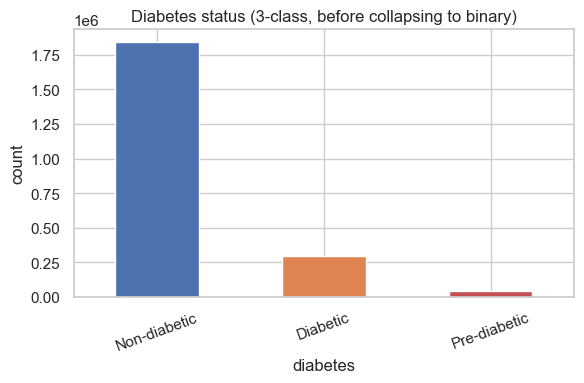
\includegraphics[width=0.55\linewidth]{images/diabetes_eda_target_3class.png}
\caption{Diabetes status, three original classes, before collapsing to
binary. Diabetic and pre-diabetic respondents are both a small minority next
to non-diabetic respondents.}
\label{fig:diabetes-eda-target}
\end{figure}

\subsection{Data understanding and cleaning}

BRFSS uses sentinel codes for "don't know" or "refused to answer" instead of
leaving a cell blank, and those codes can sit far outside the range of a real
answer. \verb|weight_00| has a large spike exactly at 999 pounds, an
essentially impossible real weight and a round, out-of-range value that would
not happen by chance in genuine data, so every \verb|weight_00 == 999| row
(153,060 rows once counted precisely) is set to missing rather than kept as a
real measurement. The same reasoning applies to \verb|bmi_00 > 100| (174,083
rows), a physically implausible body mass index. Both sentinel values are
converted to missing before the train/test split, with the actual median
imputation deferred until after the split so the imputed value is learned
from training data only.

Missingness elsewhere in the dataset has a more mundane explanation:
\verb|avg_drinks_p_day_00| is missing for 52.5\% of respondents and
\verb|poor_health_days_00| for 48.6\%, both conditionally asked questions in
the BRFSS questionnaire (average drinks per day only makes sense to ask
someone who already said they drink), so the missingness reflects survey
design, not data quality trouble. \verb|income_00| is missing for 17.8\% of
respondents, a common pattern for income questions in surveys.

Several columns turned out to be string duplicates of a clean numeric ordinal
column already present elsewhere in the table (\verb|age_group_00| next to
\verb|age_00|, \verb|education_level_00| next to \verb|education_00|,
\verb|income_level_00| next to \verb|income_00|, \verb|general_health_00|
next to \verb|gen_health_00|, \verb|last_checkup_00| next to
\verb|l_checkup_00|); keeping both would either double-count the same signal
or require re-encoding the string version from scratch for no benefit, so the
five string duplicates are dropped and the numeric ordinal versions are kept.

Exploratory analysis confirmed clinical relationships the model is expected to
pick up on. Median BMI climbs from non-diabetic to pre-diabetic to diabetic
respondents (Figure \ref{fig:diabetes-eda-bmi}), matching the established link
between excess body weight and type 2 diabetes risk. Self-reported general
health moves almost monotonically with diabetes status (Figure
\ref{fig:diabetes-eda-genhealth}): respondents rating their health
"excellent" report diabetes or pre-diabetes at a much lower rate than those
rating it "poor," which is also why this ordinal field is kept as a numeric
code rather than one-hot encoded, since the ordering itself carries signal.
The diabetic-or-pre-diabetic rate by survey year (Figure
\ref{fig:diabetes-eda-year}) drifts mildly across the five years, from
15.20\% (2020) to 15.97\% (2018), too small a gap on its own to argue
strongly for keeping \verb|year| as a feature, but kept anyway since it is
one of the few signals left carrying any residual survey-wave information
once \verb|high_bp_00| and \verb|high_cholesterol_00| had to be dropped for
the schema mismatch described in Section \ref{sec:diabetes}.

\begin{figure}[H]
\centering
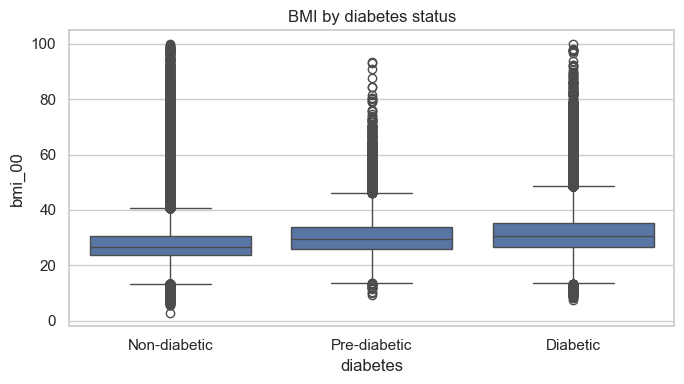
\includegraphics[width=0.55\linewidth]{images/diabetes_eda_bmi.png}
\caption{BMI by diabetes status. Median BMI rises step by step from
non-diabetic to pre-diabetic to diabetic.}
\label{fig:diabetes-eda-bmi}
\end{figure}

\begin{figure}[H]
\centering
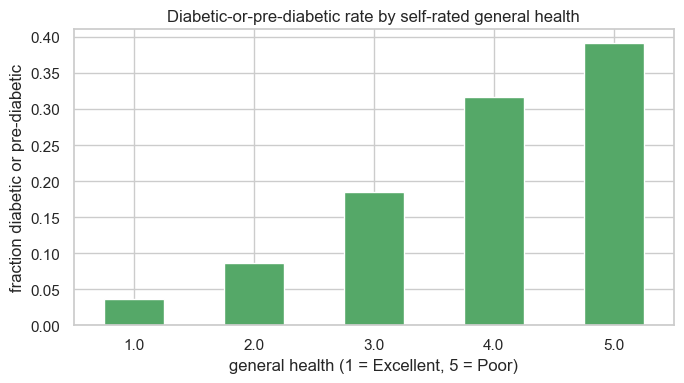
\includegraphics[width=0.55\linewidth]{images/diabetes_eda_genhealth.png}
\caption{Diabetic-or-pre-diabetic rate by self-rated general health (1 =
Excellent through 5 = Poor). The rate rises steadily from Excellent to Poor.}
\label{fig:diabetes-eda-genhealth}
\end{figure}

\begin{figure}[H]
\centering
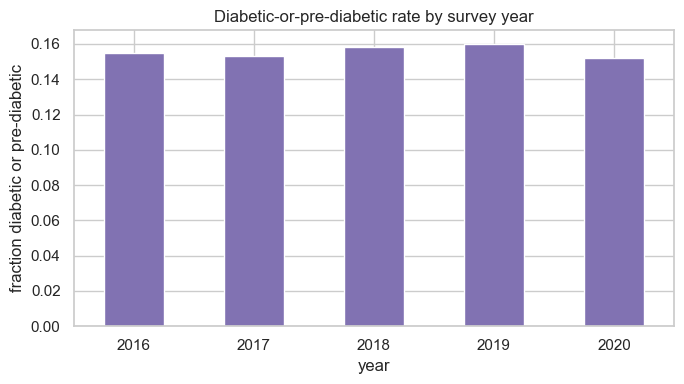
\includegraphics[width=0.55\linewidth]{images/diabetes_eda_year.png}
\caption{Diabetic-or-pre-diabetic rate by survey year, 2016-2020. The rate
drifts mildly rather than sitting flat, the reason \code{year} is kept as a
feature rather than dropped.}
\label{fig:diabetes-eda-year}
\end{figure}

\subsection{Representation}

The remaining columns fall into three groups, each needing a different
treatment before a neural network can use them. Eight genuinely two-valued
columns (sex, exercise, smoking history, alcohol use, personal history of
stroke, heart attack, or coronary disease, cost barrier to care) map directly
onto 0/1 with no information lost. Four genuinely unordered categorical
columns (race, marital status, employment status, personal-doctor access)
are one-hot encoded, since turning "Married" into a single ordinal number
would imply an ordering between marital statuses that does not exist; this
produces 29 one-hot columns. The remaining 13 numeric columns, the ordinal
survey codes (general health, education level) alongside genuinely continuous
measurements (BMI, weight, height) and \verb|year| itself, all go into one
\code{StandardScaler} group fit on the training split only.

\verb|year| is deliberately included in that scaled numeric group rather than
left as the raw calendar integer. Left unscaled, \verb|year| (2016 through
2020) would sit at a scale several times larger than every other feature,
dominating the first layer's weighted sum before training has any real
chance to learn something better than always predicting the majority class.
Standardizing it alongside the other numeric columns removes that risk
without discarding whatever residual survey-wave signal it carries.

This produces a feature matrix of width \textbf{50} (8 binary $+$ 29 one-hot
$+$ 13 standardized numeric). The 80/20 stratified split
(\code{RANDOM\_SEED = 42}) gives 1,744,900 training rows and 436,225 test
rows, with the 15.56\% positive rate preserved in both splits.

Because the target is imbalanced, a plain fit would be trained to minimize an
average loss dominated almost entirely by the majority class. Balanced sample
weights, $w = n_{\text{total}} / (2 \times n_{\text{class}})$, give
$w_{\text{neg}} = 0.5922$ and $w_{\text{pos}} = 3.2126$, so a mistake on a
diabetic row costs roughly 5.4 times as much in the training objective as a
mistake on a non-diabetic row. All three implementations apply this same
balanced weighting, though, as Section \ref{sec:diabetes-compare} shows, not
through identical mechanics underneath a shared name.

\subsection{Shared architecture}

All three implementations build the same network, computed at runtime from
the confirmed input width $d = 50$ rather than hardcoded:
\[
50 \to \text{Linear}(32) \to \text{ReLU} \to \text{Linear}(16) \to \text{ReLU}
\to \text{Linear}(1) \to \text{Sigmoid}
\]
with shape trace, for a batch of size $B$:
\[
(B, 50) \to (B, 32) \to (B, 32) \to (B, 16) \to (B, 16) \to (B, 1) \to (B, 1)
\]
Batch size 2048, 25 epochs, learning rate 0.1, and plain SGD (no momentum, no
Adam) are fixed once here and reused unchanged by all three implementations,
so the optimizer's own update rule is identical across all three rather than
needing a from-scratch Adam implementation to keep the comparison fair.

\subsection{Three implementations}

\subsubsection{From scratch, NumPy only}

Every component is an explicit Python function: \code{relu()}, a manual
\code{binary\_cross\_entropy(y\_true, y\_pred, weights=None)} that accepts the
per-row balanced weights, He-initialized weight matrices
(\code{init\_params}), an explicit \code{forward} that chains two
\code{Linear + ReLU} blocks into a final \code{Linear + Sigmoid}, and a
\code{backward} pass deriving every gradient by the chain rule, with the
balanced sample weights multiplied into the output-layer error signal
$dZ_3 = (A_3 - y) \odot w$ so imbalance correction propagates through every
downstream gradient exactly as intended. A numerical gradient check confirms
the hand-derived backward pass against a finite-difference approximation
before any full training run. Mini-batch gradient descent (batch size 2048)
trains for 25 epochs, one forward pass, one backward pass, one parameter
update per batch.

\subsubsection{TensorFlow/Keras}

The identical architecture becomes a five-line \code{Sequential} definition
(\code{Dense(32, "relu")}, \code{Dense(16, "relu")}, \code{Dense(1,
"sigmoid")}), compiled with \code{SGD(learning\_rate=0.1)} and
\code{"binary\_crossentropy"} loss, and trained with one \code{model.fit(...,
class\_weight=\{0: 0.5922, 1: 3.2126\})} call. \code{class\_weight} is Keras's
own mechanism for the same balanced weighting used by hand in scratch: it
multiplies each class's contribution to the loss by the same
\verb|weight_neg|/\verb|weight_pos| values, so this implementation trains on
the same effectively rebalanced problem as scratch, not a plain unweighted
version of it. \code{model.summary()} reports 2,177 parameters, matching the
scratch parameter count exactly and confirmed by a direct assertion in the
notebook.

\subsubsection{PyTorch}

The same architecture becomes an \code{nn.Module} (\code{DiabetesMLP}) whose
\code{forward} chains three \code{nn.Linear} layers with \code{nn.ReLU} in
between, returning raw logits with no sigmoid applied inside the module.
\code{nn.BCEWithLogitsLoss(pos\_weight=...)} applies the sigmoid and the
cross-entropy loss together in one numerically stable step, rather than
computing them separately the way scratch and Keras do, matching the
lecture's own guidance to let a framework's fused loss function handle the
activation internally. \code{pos\_weight} is set to
$w_{\text{pos}} / w_{\text{neg}} \approx 5.42$, PyTorch's own mechanism for
balanced weighting, applied to the training loop as an explicit
\code{zero\_grad} $\to$ forward $\to$ \code{loss.backward()} $\to$
\code{optimizer.step()} cycle rather than a single \code{fit()} call.
\code{torch.optim.SGD} with the same learning rate closes the loop. The
resulting parameter count, 2,177, matches both other implementations exactly.

\subsection{Component-by-implementation table}

\begin{table}[H]
\centering
\caption{Diabetes: component-by-implementation table}
\footnotesize
\begin{tabular}{@{}p{2.5cm}p{4.1cm}p{4.1cm}p{4.1cm}@{}}
\toprule
Component & Scratch & Keras & PyTorch \\
\midrule
Data loading & \code{pandas.read\_csv} $\times5$, \code{pd.concat} & same & same \\
Preprocessing & manual mean/std standardization & StandardScaler-equivalent (manual, shared) & same as scratch \\
Model definition & explicit functions $+$ a params dict & \code{Sequential([...])} & \code{nn.Module} subclass \\
Activation & \code{relu()}, \code{sigmoid()} & \code{activation="relu"/"sigmoid"} & \code{nn.ReLU()}, fused in \code{BCEWithLogitsLoss} \\
Dense/Linear layer & \code{linear()} (manual matmul) & \code{Dense(...)} & \code{nn.Linear(...)} \\
Loss & manual \code{binary\_cross\_entropy} & \code{"binary\_crossentropy"} & \code{nn.BCEWithLogitsLoss()} \\
Gradient & manual backprop & autodiff (implicit in \code{fit}) & \code{loss.backward()} (autograd) \\
Optimizer & manual \code{W -= lr * dW} & \code{optimizer="sgd"} & \code{torch.optim.SGD(...)} \\
Training loop & explicit \code{for epoch / for batch} & \code{model.fit(...)} & explicit \code{for epoch / for batch} \\
Evaluation & manual metric functions & \code{model.evaluate}-equivalent (manual) & manual (\code{model.eval()}, no-grad) \\
Prediction & \code{forward(X\_test, params)} & \code{model.predict(...)} & \code{model(x\_test)} under \code{torch.no\_grad()} \\
\bottomrule
\end{tabular}
\end{table}

\subsection{Training curves and evaluation}

\begin{figure}[H]
\centering
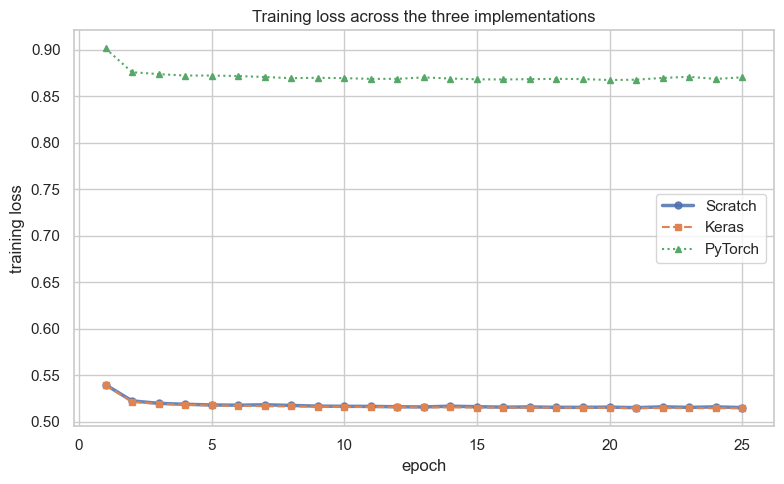
\includegraphics[width=\linewidth]{images/diabetes_compare_loss.png}
\caption{Training loss across the three implementations, one line per
implementation. Scratch and Keras track each other closely; PyTorch's curve
sits on a visibly different numeric scale for reasons explained in Section
\ref{sec:diabetes-compare}.}
\end{figure}

\begin{figure}[H]
\centering
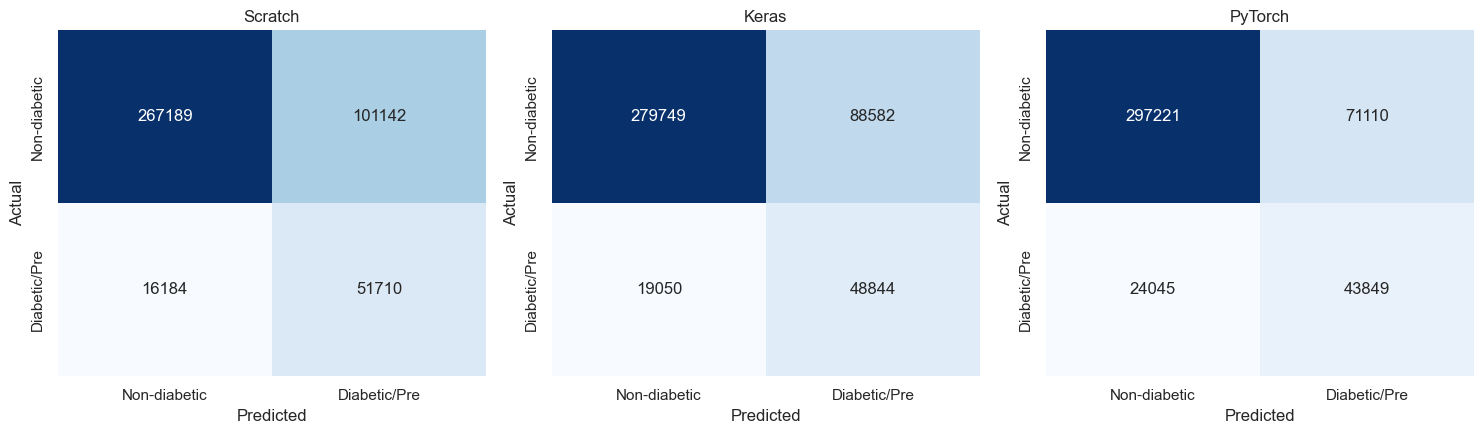
\includegraphics[width=\linewidth]{images/diabetes_compare_confmat.png}
\caption{Confusion matrices for the three implementations on the diabetes
test set (436,225 rows).}
\end{figure}

\begin{table}[H]
\centering
\caption{Diabetes: quantitative comparison, test set}
\label{tab:diabetes-quant}
\begin{tabular}{lrrrrrr}
\toprule
Implementation & Params & Train time (s) & Final loss & Accuracy & Precision & Recall \\
\midrule
Scratch & 2,177 & 69.4 & 0.5155 & 0.7310 & 0.3383 & 0.7616 \\
Keras & 2,177 & 24.7 & 0.5148 & 0.7533 & 0.3554 & 0.7194 \\
PyTorch & 2,177 & 311.0 & 0.8706 & 0.7819 & 0.3814 & 0.6458 \\
\bottomrule
\end{tabular}
\end{table}

F1 for the same three implementations, in the same order: 0.4685 (scratch),
0.4758 (Keras), 0.4796 (PyTorch).

\begin{figure}[H]
\centering

\includegraphics[width=0.6\linewidth]{images/diabetes_compare_accuracy.png}
\caption{Test accuracy by implementation.}
\end{figure}

\begin{figure}[H]
\centering

\includegraphics[width=0.7\linewidth]{images/diabetes_compare_prf1.png}
\caption{Precision, recall, and F1 by implementation. All three land in the
same 0.34-0.38 precision, 0.65-0.76 recall range, the expected footprint of
balanced weighting on an imbalanced target: more of the rare positive class
gets caught, at the cost of more false positives.}
\end{figure}

\begin{figure}[H]
\centering
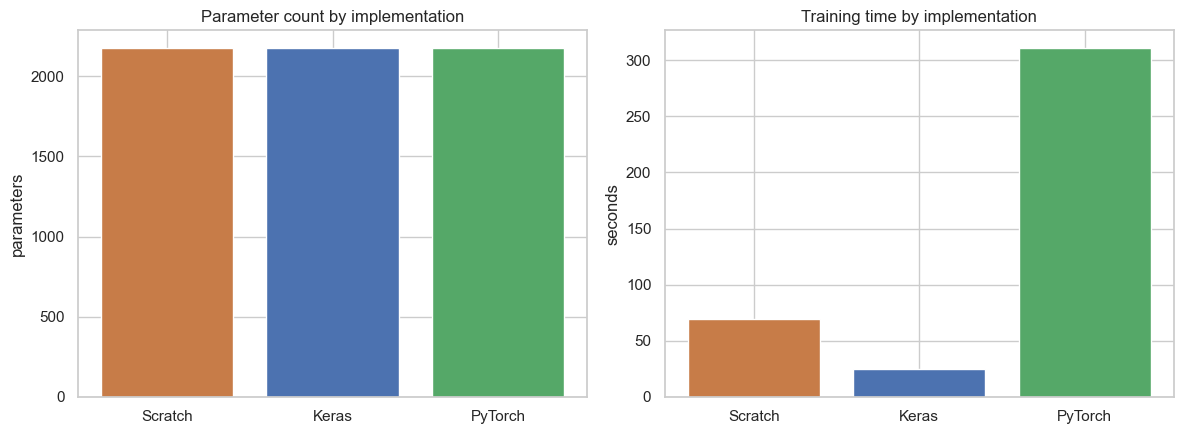
\includegraphics[width=\linewidth]{images/diabetes_compare_params_time.png}
\caption{Parameter count (identical across all three, confirming the same
architecture) and training time by implementation.}
\end{figure}

\subsection{Comparison discussion}
\label{sec:diabetes-compare}

By accuracy and F1, PyTorch comes out slightly ahead (0.782, 0.480), Keras is
close behind (0.753, 0.476), and scratch trails by a similar small margin
(0.731, 0.469). All three land within about five points of each other on both
metrics, the expected outcome for three implementations of the same
architecture trained on the same data with the same hyperparameters: the gap
is small enough to plausibly come from framework-level details (default
numerical precision, exactly how each framework shuffles batches, small
differences in how the balanced weighting is applied) rather than from one
implementation being a meaningfully better model than the others.

One number in Table \ref{tab:diabetes-quant} is genuinely not comparable
across implementations, and it is worth explaining rather than glossing over:
the final training loss. Scratch and Keras both land around 0.51, while
PyTorch sits at 0.87, a difference far bigger than the accuracy gap would
suggest. The gap comes entirely from how each implementation applies balanced
class weighting, not from PyTorch training worse. Scratch and Keras both
scale \textit{every} row's loss, multiplying the negative class's rows by
$w_{\text{neg}} = 0.5922$ and the positive class's rows by
$w_{\text{pos}} = 3.2126$, which keeps the loss on roughly the same numeric
scale an unweighted loss would have had. PyTorch's
\code{BCEWithLogitsLoss(pos\_weight=...)} only scales the positive class's
term, by the ratio $w_{\text{pos}} / w_{\text{neg}} \approx 5.42$, leaving the
negative class's term unscaled. That is a legitimate, common way to apply
class weighting in PyTorch, but it produces a loss value on a different
scale, not a directly comparable number. This is exactly the kind of
implementation-level detail this assignment is built to surface: three
frameworks offering "the same" class-weighting feature under names that
suggest equivalence (\code{class\_weight}, a \code{weights} argument,
\code{pos\_weight}), while actually parameterizing it differently underneath.

Training time tells a different story than accuracy does. Keras was fastest
(24.7s), scratch was next (69.4s), and PyTorch was noticeably slower (311.0s),
close to four and a half times scratch's time for a network with only 2,177
parameters. This lines up with how each implementation spends its time:
Keras's \code{fit()} runs its training loop in a compiled graph with very
little Python overhead per batch; scratch's mini-batch loop is plain Python,
but each batch does only a handful of matrix multiplications on a tiny
network, so the NumPy calls themselves dominate over the loop overhead;
PyTorch's per-batch loop involves autograd graph construction and teardown on
every step, a fairly fixed per-batch cost that matters far more for a network
this small than it would for a larger one where the actual computation would
dominate instead. PyTorch's flexibility, an explicit, inspectable training
loop with autograd, comes with a real per-step overhead that a network this
size cannot amortize away, a trade-off that looks very different once real
convolutions enter the picture in Sections \ref{sec:fashion} and
\ref{sec:cifar10}.

Which framework hid the most, and which gave the most control: Keras hid
essentially everything here too, the loss computation, the class-weighting
mechanics, the backward pass, and the training loop are all one
\code{compile()} call and one \code{fit()} call. PyTorch hid only the
backward pass, keeping the training loop and the loss-weighting mechanism
explicit, and that explicitness is exactly what surfaced the
\code{pos\_weight} asymmetry above, a detail that would have been invisible
inside a packaged \code{fit()} call. Scratch hid nothing, at the direct cost
of being the implementation with the most code to write and debug.

\newpage
% ---------------------------------------------------------------------
\section{Fashion-MNIST: 10-Class Image Classification (CNN)}
\label{sec:fashion}
% ---------------------------------------------------------------------

\subsection{Problem description}

This application classifies a $28\times28$ grayscale image of a clothing item
into one of ten categories (T-shirt/top, trouser, pullover, dress, coat,
sandal, shirt, sneaker, bag, ankle boot). Unlike the diabetes application,
the input here has real 2-D spatial structure, neighboring pixels are
related, and a shape like a sleeve or a shoe sole is a local pattern that
recurs at different positions across the image, exactly the setting Lecture
04 gives for why a CNN, not an MLP, is the right architecture: local
connectivity and weight sharing let a small set of learned kernels detect the
same pattern anywhere in the image.

\subsection{Dataset}

Fashion-MNIST is loaded via \code{keras.datasets.fashion\_mnist.load\_data()},
which downloads and caches the dataset automatically on first use, no manual
file management required. It ships as 60,000 training images and 10,000 test
images, each $28\times28$ pixels, single channel, pixel values in $[0, 255]$
before normalization. Every one of the ten classes has exactly 6,000 training
images and 1,000 test images (Figure \ref{fig:fm-eda-balance}), a
deliberately balanced benchmark dataset, so no class-imbalance correction is
needed here, unlike the diabetes application: a model that always predicted
one class would score only 10\% accuracy, not a deceptively high number the
way it would on an imbalanced target.

\begin{figure}[H]
\centering
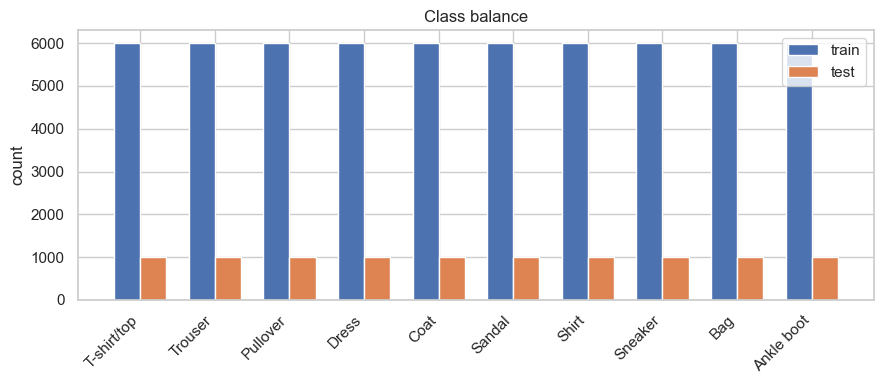
\includegraphics[width=0.7\linewidth]{images/fashion_mnist_eda_class_balance.png}
\caption{Fashion-MNIST class balance, train and test. Every class has exactly
6,000 training and 1,000 test images.}
\label{fig:fm-eda-balance}
\end{figure}

\begin{figure}[H]
\centering
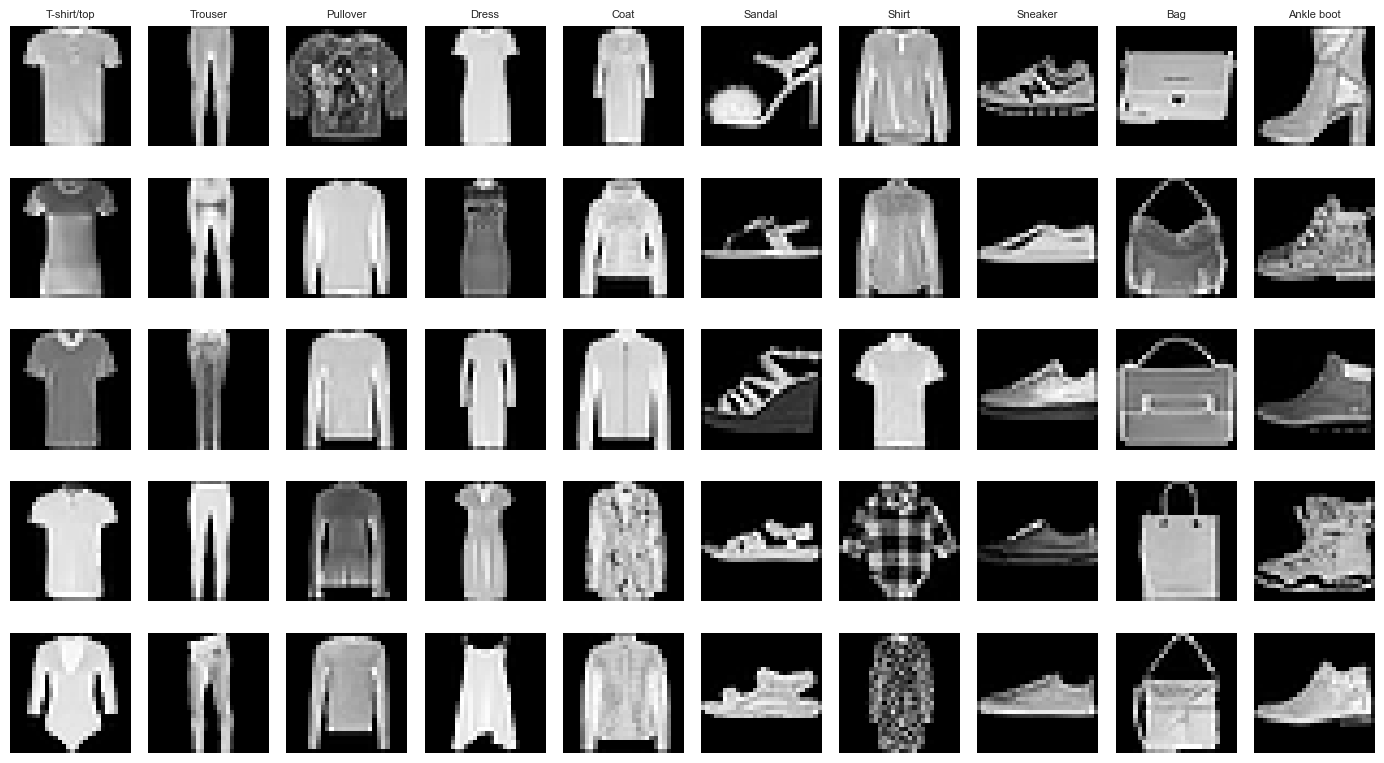
\includegraphics[width=\linewidth]{images/fashion_mnist_eda_sample_grid.png}
\caption{Five sample images per class. The classes are visually distinct in
obvious cases and genuinely similar in others (shirt vs. pullover vs. coat),
which is a reasonable source of the classification errors seen later.}
\end{figure}

\begin{figure}[H]
\centering
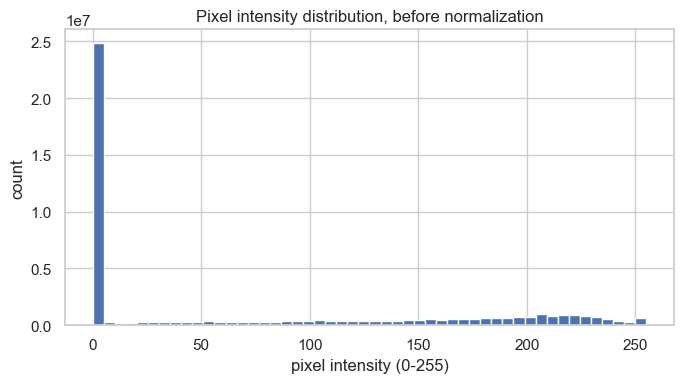
\includegraphics[width=0.6\linewidth]{images/fashion_mnist_eda_pixel_hist.png}
\caption{Pixel intensity distribution before normalization. The large spike
at 0 reflects how much of every image is plain black background around a
centered clothing item.}
\end{figure}

\subsection{Representation}

Pixel values are cast to \code{float32} and divided by 255, mapping the
$[0,255]$ integer range to $[0,1]$. Two array layouts are kept side by side
for the rest of the notebook: channel-first, $(N, 1, 28, 28)$, for scratch and
PyTorch, and channel-last, $(N, 28, 28, 1)$, for Keras's default convolution
layout. No further cleaning is needed, since this is a curated benchmark
dataset with no missing values, no sentinel codes, and no schema
inconsistencies to resolve.

\subsection{Shared architecture}

All three implementations build the same network:
\[
\resizebox{\linewidth}{!}{$28\times28\times1 \to \text{Conv}(1{\to}32, k{=}3, \text{pad}{=}1) \to \text{ReLU}
\to \text{MaxPool}(2) \to \text{Conv}(32{\to}64, k{=}3, \text{pad}{=}1) \to
\text{ReLU} \to \text{MaxPool}(2)$}
\]
\[
\to \text{Flatten} (64{\times}7{\times}7 = 3136) \to \text{Linear}(3136{\to}128)
\to \text{ReLU} \to \text{Linear}(128{\to}10)
\]
with shape trace, for a batch of size $B$:
\[
\resizebox{\linewidth}{!}{$(B,1,28,28) \to (B,32,28,28) \to (B,32,14,14) \to (B,64,14,14) \to (B,64,7,7)
\to (B,3136) \to (B,128) \to (B,10)$}
\]
Batch size 256, 10 epochs, learning rate 0.05, and plain SGD are fixed once
here and reused unchanged across all three implementations.

\subsection{Three implementations}

\subsubsection{From scratch, NumPy only}

Every operation, convolution, pooling, the dense layers, the loss, and every
gradient, is implemented by hand. Convolution is the operation worth being
concrete about: a $3\times3$ kernel is lined up against a $3\times3$ image
patch, the nine overlapping (kernel value, pixel) pairs are multiplied and
summed into one output value, and the kernel slides across every position to
build the full feature map, the same kernel reused at every position, weight
sharing, which is what lets one small kernel generalize across the whole
image instead of only recognizing a pattern in the one spot it happened to be
trained on. A direct position-by-position loop implementing that operation
was too slow to be practical, the second convolutional layer alone took over
two seconds per batch on this network's real layer sizes, so the notebook's
\code{conv2d\_forward}/\code{conv2d\_backward} instead use an \code{im2col}
approach: every patch the kernel will ever touch is extracted up front as a
zero-copy strided view and stacked into one matrix, turning the whole
convolution into a single matrix multiplication, the exact same computation
as the naive loop, done for every position simultaneously rather than one at
a time, about 40 times faster on this network's real layer sizes. A numerical
gradient check confirms the hand-derived convolution and pooling backward
passes against a finite-difference approximation before any full training
run; this check caught a real bug during development, a redundant
$1/N$ division in the dense-layer backward pass that had been silently
shrinking every dense-layer gradient (convolution-layer gradients, computed
by a different code path with no such division, were unaffected), fixed
before the results reported below were produced. Mini-batch gradient descent
(batch size 256, 235 batches per epoch) trains for 10 epochs.

\subsubsection{TensorFlow/Keras}

The identical architecture becomes an eight-layer \code{Sequential}
definition (\code{Conv2D(32,3,padding="same",activation="relu")},
\code{MaxPooling2D(2)}, \code{Conv2D(64,...)}, \code{MaxPooling2D(2)},
\code{Flatten()}, \code{Dense(128,"relu")}, \code{Dense(10)}), compiled with
\code{SGD(learning\_rate=0.05)} and
\code{SparseCategoricalCrossentropy(from\_logits=True)}, trained with one
\code{model.fit(X\_train\_hwc, y\_train, batch\_size=256, epochs=10)} call.
\code{model.summary()} reports 421,642 parameters, matching scratch exactly.
The convolution and pooling loops that scratch writes out explicitly have
disappeared entirely from this implementation's own code, encapsulated
instead inside the \code{Conv2D}/\code{MaxPooling2D} layer objects.

\subsubsection{PyTorch}

The same architecture becomes an \code{nn.Module} (\code{FashionCNN}) with a
\code{self.features} block (\code{nn.Conv2d}, \code{nn.ReLU},
\code{nn.MaxPool2d}, twice) followed by a \code{self.classifier} block
(\code{nn.Flatten}, \code{nn.Linear(3136,128)}, \code{nn.ReLU},
\code{nn.Linear(128,10)}), returning raw logits consumed by
\code{nn.CrossEntropyLoss()}. The training loop stays explicit
(\code{zero\_grad} $\to$ forward $\to$ loss $\to$ \code{backward()} $\to$
\code{optimizer.step()}), with \code{torch.optim.SGD} at the same learning
rate. The resulting parameter count, 421,642, matches both other
implementations exactly, confirmed by a direct assertion in the notebook.

\subsection{Component-by-implementation table}

\begin{table}[H]
\centering
\caption{Fashion-MNIST: component-by-implementation table}
\footnotesize
\begin{tabular}{@{}p{2.5cm}p{4.1cm}p{4.1cm}p{4.1cm}@{}}
\toprule
Component & Scratch & Keras & PyTorch \\
\midrule
Data loading & Keras loader, shared NumPy arrays & same & same \\
Preprocessing & manual /255, channel-first reshape & /255, channel-last (default) & /255, channel-first \\
Model definition & explicit functions $+$ a params dict & \code{Sequential([...])} & \code{nn.Module} subclass \\
Convolution & \code{conv2d\_forward}/\code{backward} (\code{im2col}) & \code{Conv2D(...)} & \code{nn.Conv2d(...)} \\
Activation & \code{relu()} & \code{activation="relu"} & \code{nn.ReLU()} \\
Pooling & \code{max\_pool2d\_forward}/\code{backward} & \code{MaxPooling2D(2)} & \code{nn.MaxPool2d(2)} \\
Flatten & \code{flatten\_forward}/\code{backward} (reshape) & \code{Flatten()} & \code{nn.Flatten()} \\
Dense/Linear layer & \code{linear\_forward}/\code{backward} & \code{Dense(...)} & \code{nn.Linear(...)} \\
Loss & manual softmax cross-entropy & \code{SparseCategorical}\allowbreak\code{Crossentropy(}\allowbreak\code{from\_logits=True)} & \code{nn.CrossEntropyLoss()} \\
Gradient & manual backprop & autodiff (implicit in \code{fit}) & \code{loss.backward()} (autograd) \\
Optimizer & manual \code{W -= lr * dW} & \code{optimizer="sgd"} & \code{torch.optim.SGD(...)} \\
Training loop & explicit \code{for epoch / for batch} & \code{model.fit(...)} & explicit \code{for epoch / for batch} \\
Evaluation & manual metric functions & \code{model.evaluate}-equivalent (manual) & manual (\code{model.eval()}, no-grad) \\
Prediction & \code{forward(X\_test, params)} & \code{model.predict(...)} & \code{model(x\_test)} under \code{torch.no\_grad()} \\
\bottomrule
\end{tabular}
\end{table}

\subsection{Training curves and evaluation}

\begin{figure}[H]
\centering
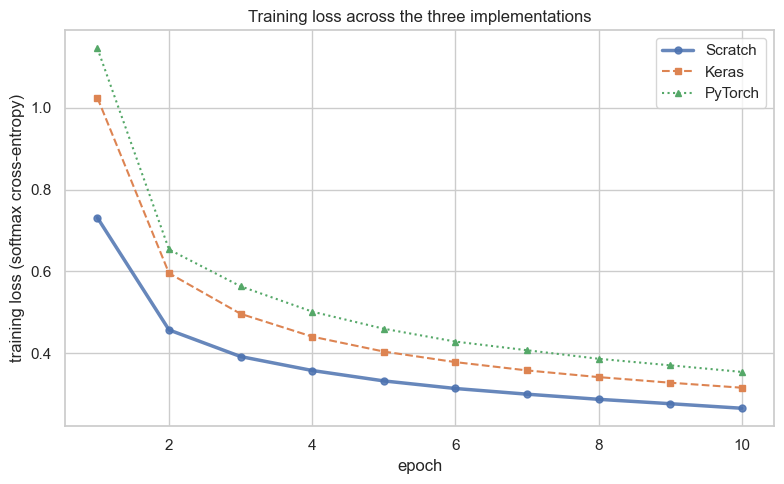
\includegraphics[width=\linewidth]{images/fashion_mnist_compare_loss.png}
\caption{Training loss across the three implementations.}
\end{figure}

\begin{figure}[H]
\centering
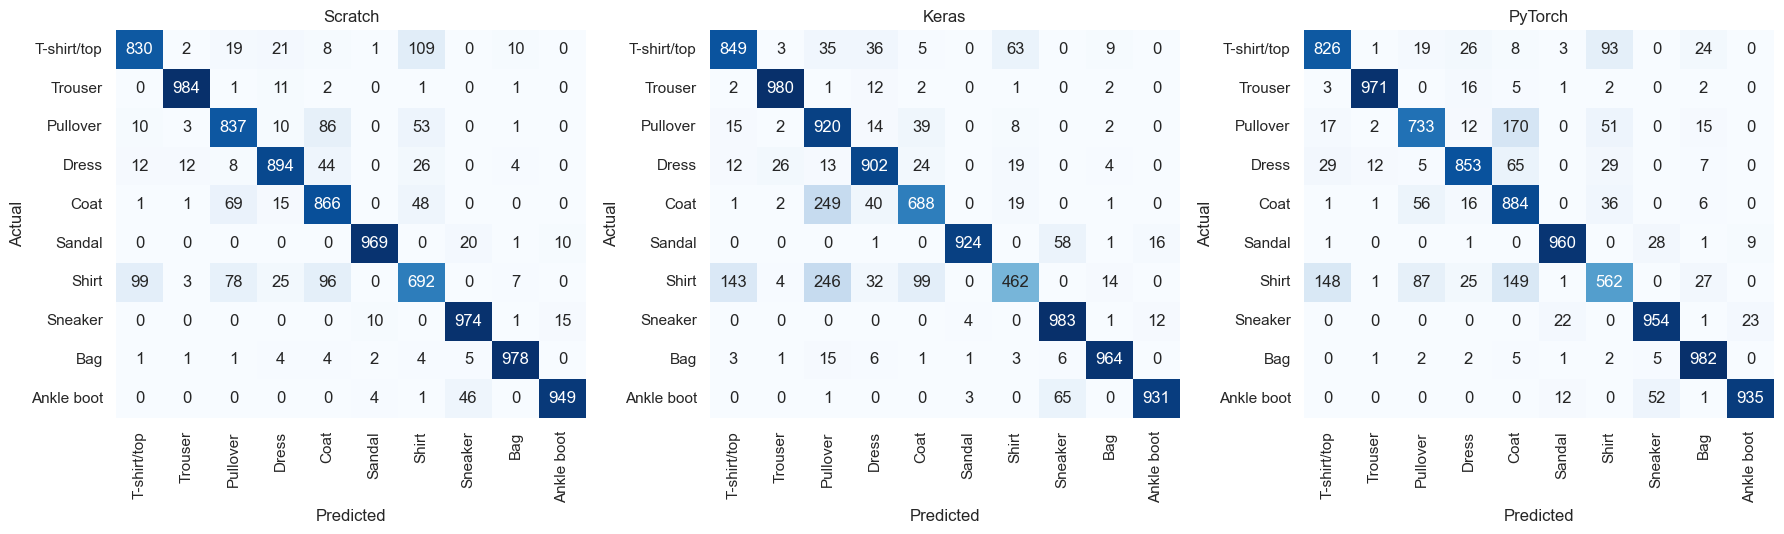
\includegraphics[width=\linewidth]{images/fashion_mnist_compare_confmat.png}
\caption{Confusion matrices for the three implementations on the Fashion-MNIST
test set (10,000 images). The shirt/pullover/coat cluster is the most common
source of confusion in all three, consistent with how visually similar those
classes are (Figure \ref{fig:fm-eda-balance}'s neighboring figure).}
\end{figure}

\begin{table}[H]
\centering
\caption{Fashion-MNIST: quantitative comparison, test set}
\label{tab:fm-quant}
\begin{tabular}{lrrrrrr}
\toprule
Implementation & Params & Train time (s) & Final loss & Accuracy & Precision (macro) & Recall (macro) \\
\midrule
Scratch & 421,642 & 1,330.5 & 0.2655 & 0.8973 & 0.8976 & 0.8973 \\
Keras & 421,642 & 75.6 & 0.3157 & 0.8603 & 0.8695 & 0.8603 \\
PyTorch & 421,642 & 191.5 & 0.3544 & 0.8660 & 0.8676 & 0.8660 \\
\bottomrule
\end{tabular}
\end{table}

Macro F1 for the same three implementations, in the same order: 0.8970
(scratch), 0.8565 (Keras), 0.8641 (PyTorch).

\begin{figure}[H]
\centering
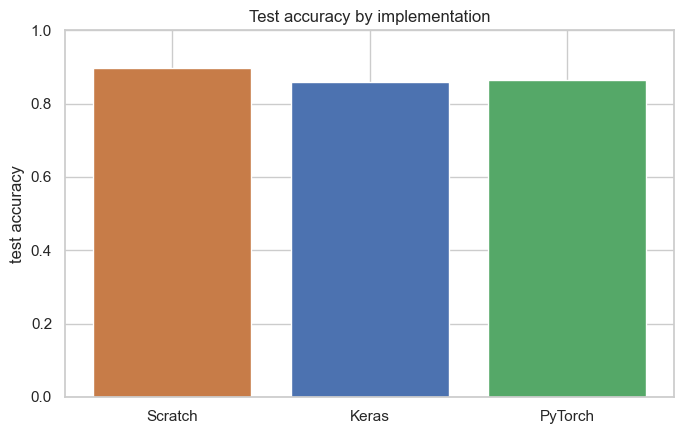
\includegraphics[width=0.6\linewidth]{images/fashion_mnist_compare_accuracy.png}
\caption{Test accuracy by implementation. Scratch wins here, the only
application in this report where it does.}
\end{figure}

\begin{figure}[H]
\centering
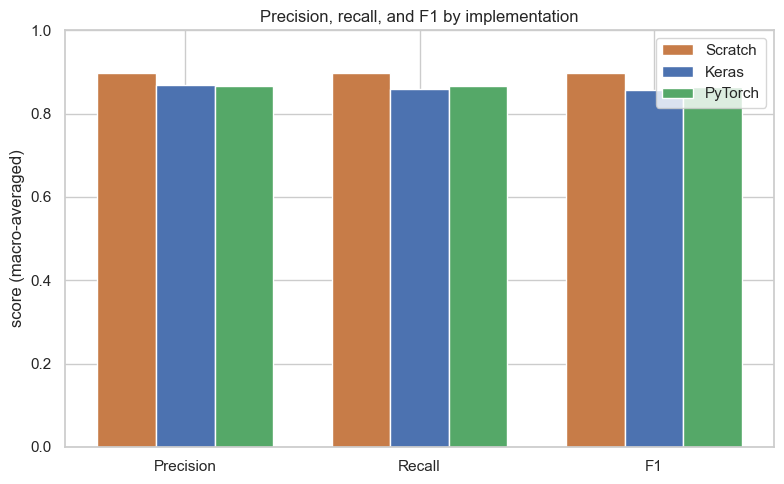
\includegraphics[width=0.7\linewidth]{images/fashion_mnist_compare_prf1.png}
\caption{Precision, recall, and F1 (macro-averaged) by implementation.}
\end{figure}

\begin{figure}[H]
\centering
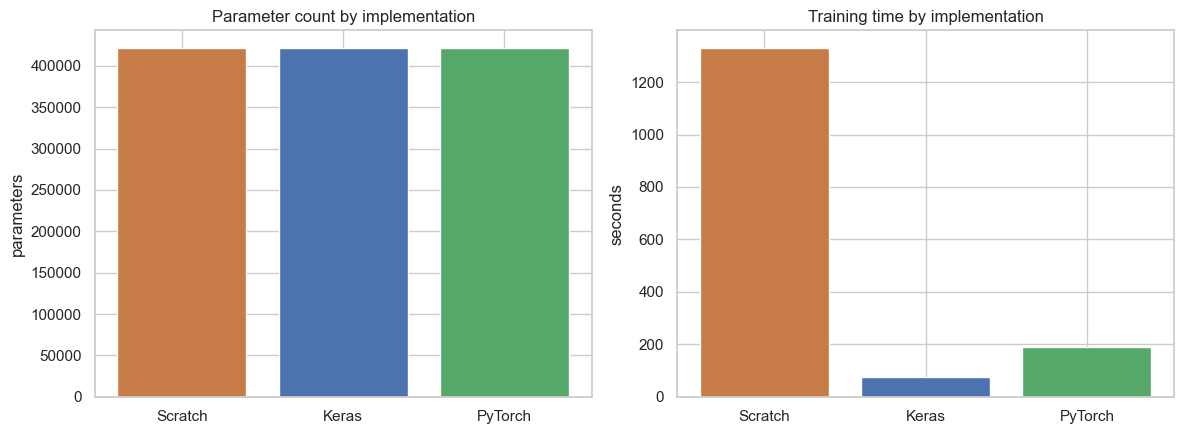
\includegraphics[width=\linewidth]{images/fashion_mnist_compare_params_time.png}
\caption{Parameter count (identical across all three) and training time by
implementation. Scratch's training time is on a dramatically different scale
from the other two.}
\end{figure}

\subsection{Comparison discussion}
\label{sec:fm-compare}

By test accuracy, scratch actually comes out ahead: 0.897 against PyTorch's
0.866 and Keras's 0.860. That is a genuinely interesting result, since
scratch is not usually the implementation expected to win. The most likely
explanation is initialization and randomness, not anything about the
implementation being fundamentally better: scratch uses explicit He
initialization with a fixed seed, while Keras and PyTorch each apply their
own default initializer, also ReLU-appropriate but not guaranteed to produce
the same starting point. Ten epochs is not a lot of training, so a difference
in where each implementation starts can still show up meaningfully in where
it ends up. All three are within about four points of each other on
accuracy, small enough to be consistent with three implementations of the
same architecture rather than three genuinely different models, echoing the
diabetes application's own spread.

Training time tells the more dramatic story here. Scratch took 1,330.5
seconds (about 22 minutes), Keras took 75.6 seconds, and PyTorch took 191.5
seconds, scratch roughly 17.6 times slower than Keras and 6.9 times slower
than PyTorch. That gap makes sense given what each implementation is
actually doing under the hood: Keras's \code{fit()} runs the entire training
loop inside a compiled graph, with convolution implemented by heavily
optimized, vectorized routines and essentially no per-batch Python overhead.
PyTorch's explicit training loop carries some per-batch Python and autograd
overhead, but its convolution operation is still a compiled, optimized
routine. Scratch's \code{conv2d\_forward}/\code{conv2d\_backward}, even with
the \code{im2col} speedup over a naive position-by-position loop, are still
plain NumPy matrix multiplies issued from a Python training loop, with none
of the operator fusion or lower-level optimization a mature deep learning
framework applies to convolution specifically. The \code{im2col} rewrite
made training feasible at all; it does not close the gap with frameworks
built and optimized specifically around this operation. This is a sharp
contrast with the diabetes MLP in Section \ref{sec:diabetes-compare}, where
scratch was comparably fast to the frameworks and PyTorch was in fact the
slowest implementation: once a network's forward pass genuinely involves
convolution rather than only small dense-layer matrix multiplies, the
speed picture flips entirely.

Which framework hid the most, and which gave the most control: Keras hid
essentially everything, the convolution, the pooling, the backward pass, and
the training loop are all one \code{Sequential} definition and one
\code{fit()} call. PyTorch hid the backward pass via autograd but kept the
training loop and the layer composition explicit. Scratch hid nothing, every
multiply, every gradient, and every parameter update is code that was written
and can be read line by line. The cost of that visibility, in this
application, is a very real difference in wall-clock training time, exactly
the trade-off the three abstraction levels are meant to represent: more
convenience and speed at the cost of visibility, or more visibility and
control at the cost of convenience and speed.

\newpage
% ---------------------------------------------------------------------
\section{CIFAR-10: 10-Class Image Classification (CNN)}
\label{sec:cifar10}
% ---------------------------------------------------------------------

\subsection{Problem description}

This application classifies a $32\times32$ RGB color photograph into one of
ten object categories (airplane, automobile, bird, cat, deer, dog, frog,
horse, ship, truck). It uses the same architecture family as Fashion-MNIST,
a CNN, for the same reason, real 2-D spatial structure that a convolution can
exploit, but with three input channels instead of one and a task that is
substantially harder: distinguishing a cat from a dog, or an automobile from
a truck, in a real photograph compressed to $32\times32$ pixels, is a
genuinely harder visual problem than distinguishing clothing silhouettes on a
plain background.

\subsection{Dataset}

CIFAR-10 is loaded via \code{keras.datasets.cifar10.load\_data()}, which
downloads and caches the dataset automatically on first use ($\sim$170MB, a
one-time download). It ships as 50,000 training images and 10,000 test
images, each $32\times32$ pixels, three channels, pixel values in $[0,255]$
before normalization. Every one of the ten classes has exactly 5,000 training
images and 1,000 test images, another deliberately balanced benchmark
dataset requiring no class-weighting correction.

\begin{figure}[H]
\centering
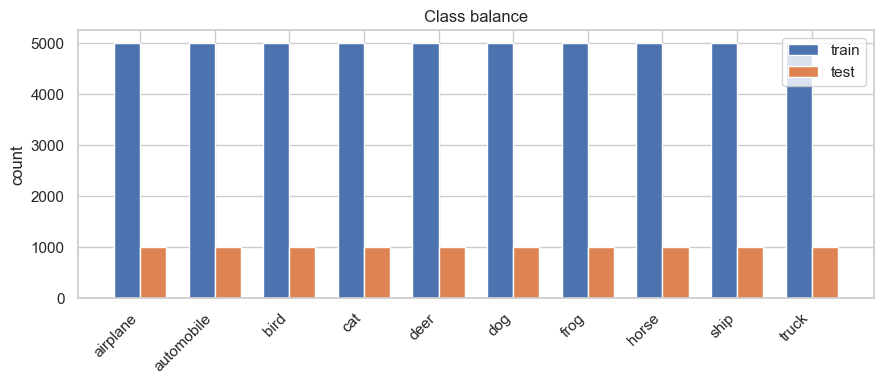
\includegraphics[width=0.7\linewidth]{images/cifar10_eda_class_balance.png}
\caption{CIFAR-10 class balance, train and test. Every class has exactly
5,000 training and 1,000 test images.}
\end{figure}

\begin{figure}[H]
\centering
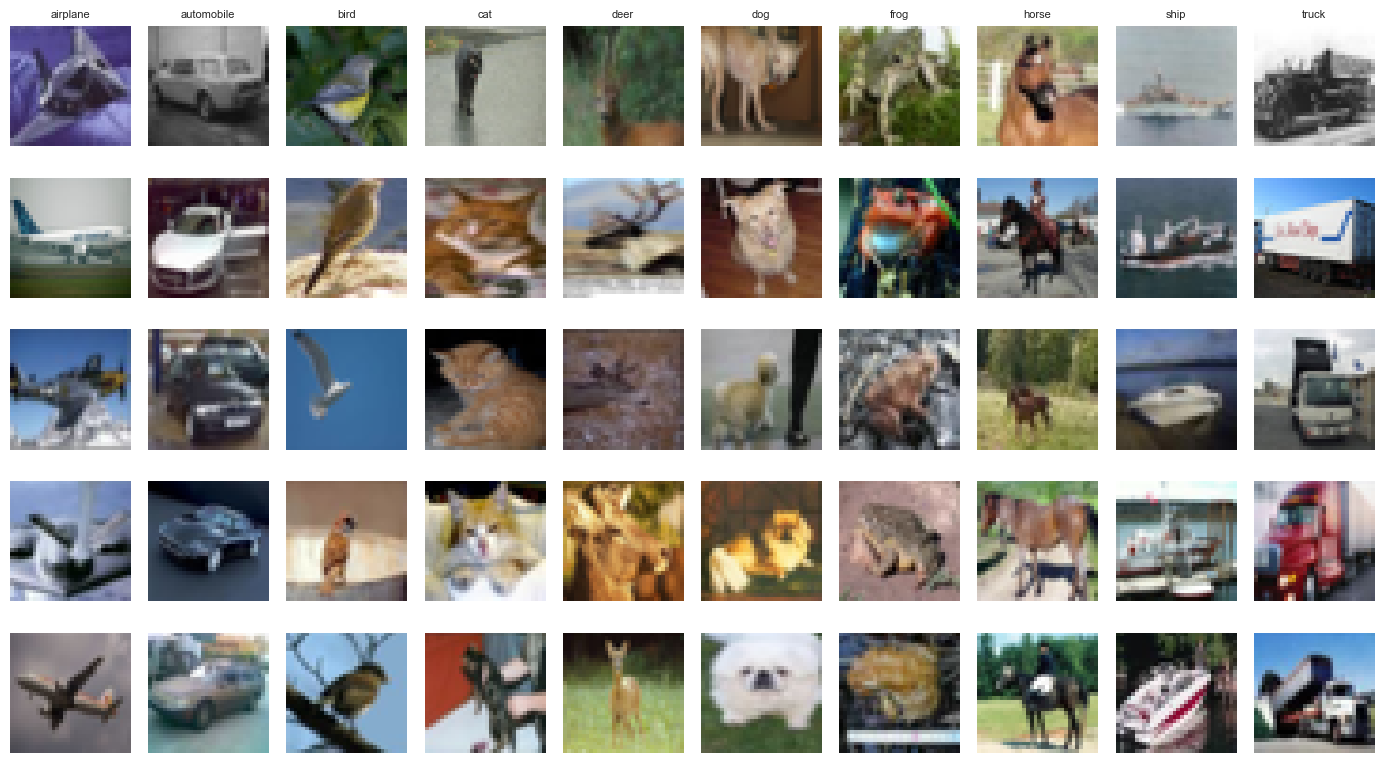
\includegraphics[width=\linewidth]{images/cifar10_eda_sample_grid.png}
\caption{Five sample images per class. These are real color photographs at
only $32\times32$ resolution, small enough that some category pairs
(automobile/truck, cat/dog) are genuinely ambiguous even to a human glance.}
\end{figure}

\begin{figure}[H]
\centering
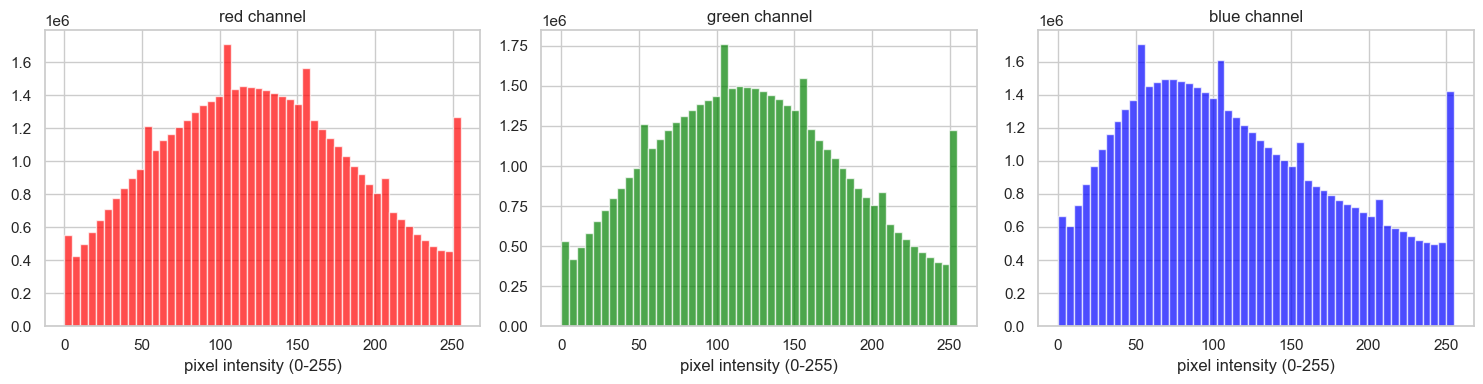
\includegraphics[width=\linewidth]{images/cifar10_eda_channel_hist.png}
\caption{Per-channel (red, green, blue) pixel intensity distribution before
normalization. All three channels span the full 0-255 range with a broadly
similar shape, unlike Fashion-MNIST's single-channel histogram, which had a
dominant spike at 0 from plain black background.}
\end{figure}

\subsection{Representation}

Pixel values are cast to \code{float32} and divided by 255. CIFAR-10 ships
channel-last, $(N, 32, 32, 3)$, matching Keras's default layout directly with
no transpose needed; scratch and PyTorch instead use a transposed
channel-first copy, $(N, 3, 32, 32)$. No further cleaning is needed, the same
curated-benchmark reasoning as Fashion-MNIST.

\subsection{Shared architecture}

All three implementations build the same network, a direct instance of the
CNN architecture the course tutorial material works out in full for a
$3\times32\times32$ input:
\[
\resizebox{\linewidth}{!}{$3\times32\times32 \to \text{Conv}(3{\to}32, k{=}3, \text{pad}{=}1) \to \text{ReLU}
\to \text{MaxPool}(2) \to \text{Conv}(32{\to}64, k{=}3, \text{pad}{=}1) \to
\text{ReLU} \to \text{MaxPool}(2)$}
\]
\[
\to \text{Flatten} (64{\times}8{\times}8 = 4096) \to \text{Linear}(4096{\to}128)
\to \text{ReLU} \to \text{Linear}(128{\to}10)
\]
with shape trace, for a batch of size $B$:
\[
\resizebox{\linewidth}{!}{$(B,3,32,32) \to (B,32,32,32) \to (B,32,16,16) \to (B,64,16,16) \to (B,64,8,8)
\to (B,4096) \to (B,128) \to (B,10)$}
\]
matching the tutorial's own worked shape progression exactly. Batch size 256,
12 epochs, learning rate 0.05, and plain SGD are fixed once here and reused
unchanged across all three implementations.

\subsection{Three implementations}

\subsubsection{From scratch, NumPy only}

The scratch implementation reuses the same \code{conv2d\_forward}/
\code{backward} (\code{im2col}), \code{max\_pool2d\_forward}/\code{backward},
\code{relu()}, and softmax-cross-entropy machinery built for Fashion-MNIST,
made explicitly 3-channel-aware: the first kernel's shape is
$(32, 3, 3, 3)$ rather than $(32, 1, 3, 3)$, since the input now has three
input channels instead of one. A numerical gradient check on a synthetic
3-input-channel sample confirms the convolution backward pass is correct
specifically for the multi-channel case, not only the single-channel case
Fashion-MNIST exercised, before any full training run. The same redundant
$1/N$ dense-layer division bug fixed for Fashion-MNIST was fixed here too,
before this notebook was ever executed, so no training run here was affected
by it. Mini-batch gradient descent (batch size 256, 196 batches per epoch)
trains for 12 epochs.

\subsubsection{TensorFlow/Keras}

The identical architecture becomes the same eight-layer \code{Sequential}
shape as Fashion-MNIST, with \code{Conv2D(32,3,...)} taking a
$(32,32,3)$ input directly, no channel-order conversion needed since CIFAR-10
already ships in Keras's preferred layout. Compiled with
\code{SGD(learning\_rate=0.05)} and
\code{SparseCategoricalCrossentropy(from\_logits=True)}, trained with one
\code{model.fit(X\_train\_hwc, y\_train, batch\_size=256, epochs=12)} call.
\code{model.summary()} reports 545,098 parameters, matching scratch exactly.

\subsubsection{PyTorch}

The same architecture becomes an \code{nn.Module} (\code{Cifar10CNN}),
structurally identical to Fashion-MNIST's \code{FashionCNN} except for the
first convolution's input channel count (3 instead of 1) and the flattened
feature size ($64 \times 8 \times 8 = 4096$ instead of $64 \times 7 \times 7 =
3136$, since CIFAR-10's larger $32\times32$ input survives two
stride-2 poolings at a larger spatial size than Fashion-MNIST's $28\times28$
does). The explicit training loop and \code{nn.CrossEntropyLoss()} carry over
unchanged from Fashion-MNIST. The resulting parameter count, 545,098, matches
both other implementations exactly.

\subsection{Component-by-implementation table}

\begin{table}[H]
\centering
\caption{CIFAR-10: component-by-implementation table}
\footnotesize
\begin{tabular}{@{}p{2.5cm}p{4.1cm}p{4.1cm}p{4.1cm}@{}}
\toprule
Component & Scratch & Keras & PyTorch \\
\midrule
Data loading & Keras loader, shared NumPy arrays & same & same \\
Preprocessing & manual /255, channel-first reshape & /255, channel-last (as shipped, no transpose) & /255, channel-first (transposed) \\
Model definition & explicit functions $+$ a params dict & \code{Sequential([...])} & \code{nn.Module} subclass \\
Convolution & \code{conv2d\_forward}/\code{backward} (\code{im2col}, 3-channel-aware) & \code{Conv2D(...)} & \code{nn.Conv2d(...)} \\
Activation & \code{relu()} & \code{activation="relu"} & \code{nn.ReLU()} \\
Pooling & \code{max\_pool2d\_forward}/\code{backward} & \code{MaxPooling2D(2)} & \code{nn.MaxPool2d(2)} \\
Flatten & \code{flatten\_forward}/\code{backward} (reshape) & \code{Flatten()} & \code{nn.Flatten()} \\
Dense/Linear layer & \code{linear\_forward}/\code{backward} & \code{Dense(...)} & \code{nn.Linear(...)} \\
Loss & manual softmax cross-entropy & \code{SparseCategorical}\allowbreak\code{Crossentropy(}\allowbreak\code{from\_logits=True)} & \code{nn.CrossEntropyLoss()} \\
Gradient & manual backprop & autodiff (implicit in \code{fit}) & \code{loss.backward()} (autograd) \\
Optimizer & manual \code{W -= lr * dW} & \code{optimizer="sgd"} & \code{torch.optim.SGD(...)} \\
Training loop & explicit \code{for epoch / for batch} & \code{model.fit(...)} & explicit \code{for epoch / for batch} \\
Evaluation & manual metric functions & \code{model.evaluate}-equivalent (manual) & manual (\code{model.eval()}, no-grad) \\
Prediction & \code{forward(X\_test, params)} & \code{model.predict(...)} & \code{model(x\_test)} under \code{torch.no\_grad()} \\
\bottomrule
\end{tabular}
\end{table}

\subsection{Training curves and evaluation}

\begin{figure}[H]
\centering
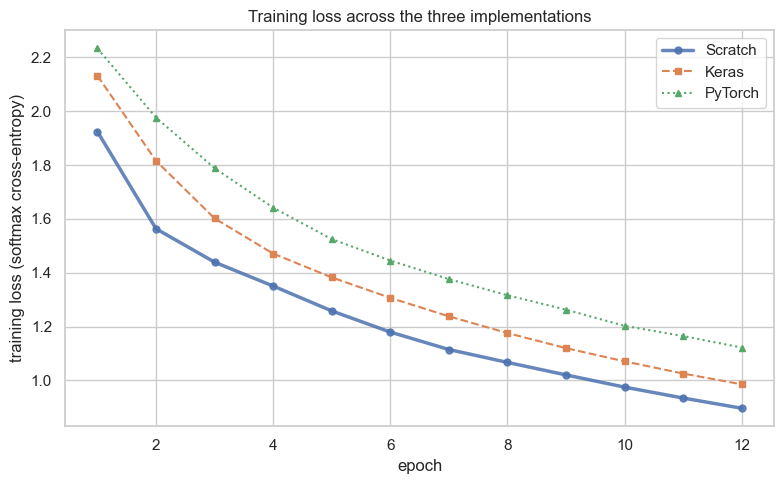
\includegraphics[width=\linewidth]{images/cifar10_compare_loss.png}
\caption{Training loss across the three implementations.}
\end{figure}

\begin{figure}[H]
\centering
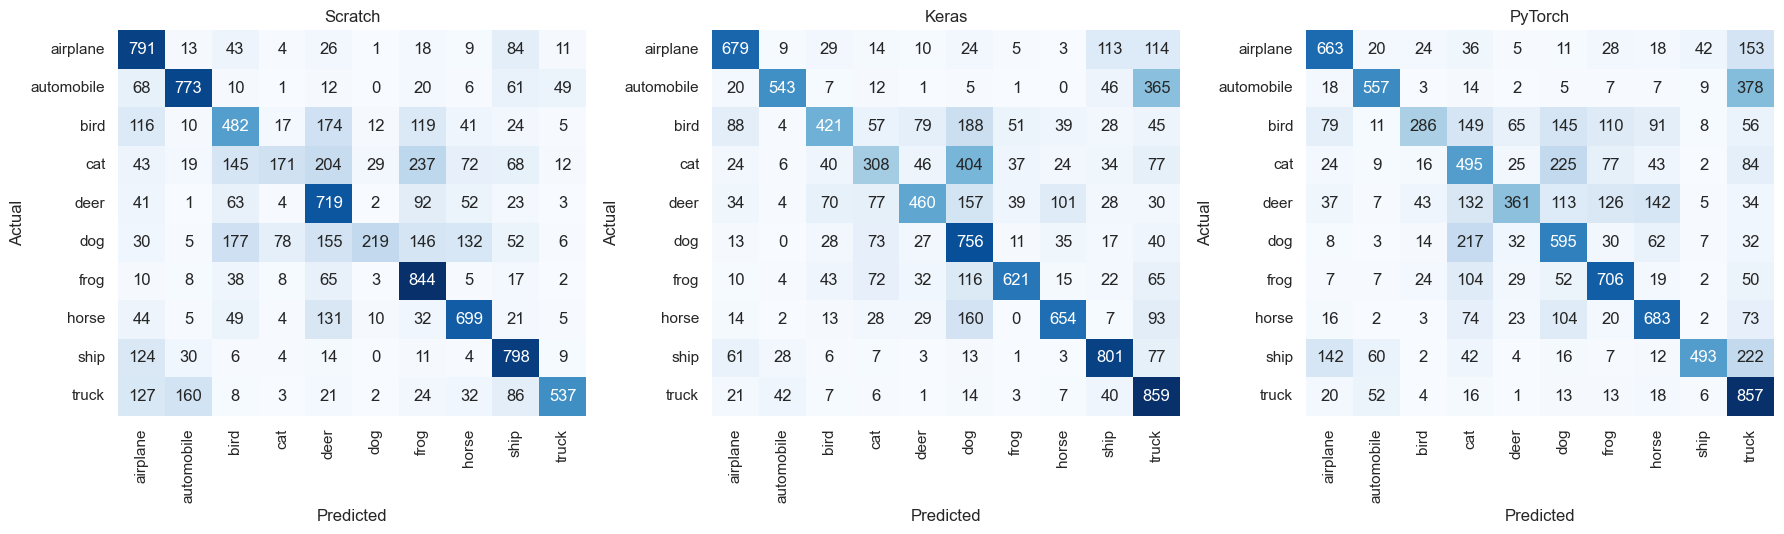
\includegraphics[width=\linewidth]{images/cifar10_compare_confmat.png}
\caption{Confusion matrices for the three implementations on the CIFAR-10
test set (10,000 images). Cat/dog and automobile/truck are the most commonly
confused pairs in all three, consistent with the visual ambiguity noted in
the sample grid above.}
\end{figure}

\begin{table}[H]
\centering
\caption{CIFAR-10: quantitative comparison, test set}
\label{tab:cifar-quant}
\begin{tabular}{lrrrrrr}
\toprule
Implementation & Params & Train time (s) & Final loss & Accuracy & Precision (macro) & Recall (macro) \\
\midrule
Scratch & 545,098 & 1,875.8 & 0.8965 & 0.6033 & 0.6335 & 0.6033 \\
Keras & 545,098 & 103.3 & 0.9854 & 0.6102 & 0.6477 & 0.6102 \\
PyTorch & 545,098 & 244.1 & 1.1220 & 0.5696 & 0.6163 & 0.5696 \\
\bottomrule
\end{tabular}
\end{table}

Macro F1 for the same three implementations, in the same order: 0.5794
(scratch), 0.6078 (Keras), 0.5655 (PyTorch).

\begin{figure}[H]
\centering
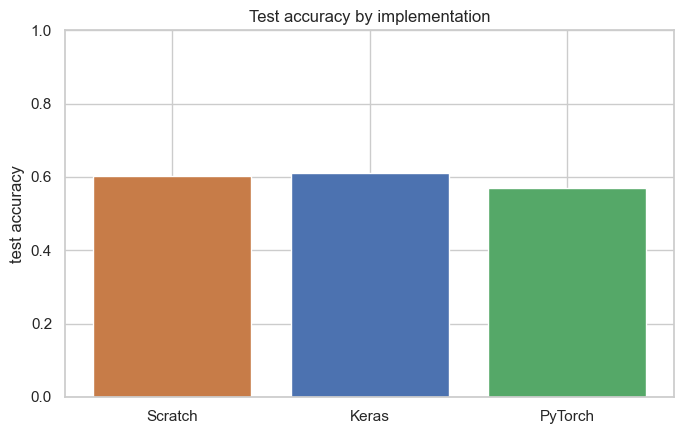
\includegraphics[width=0.6\linewidth]{images/cifar10_compare_accuracy.png}
\caption{Test accuracy by implementation. Absolute accuracy is much lower
than Fashion-MNIST's, the expected effect of a genuinely harder task.}
\end{figure}

\begin{figure}[H]
\centering
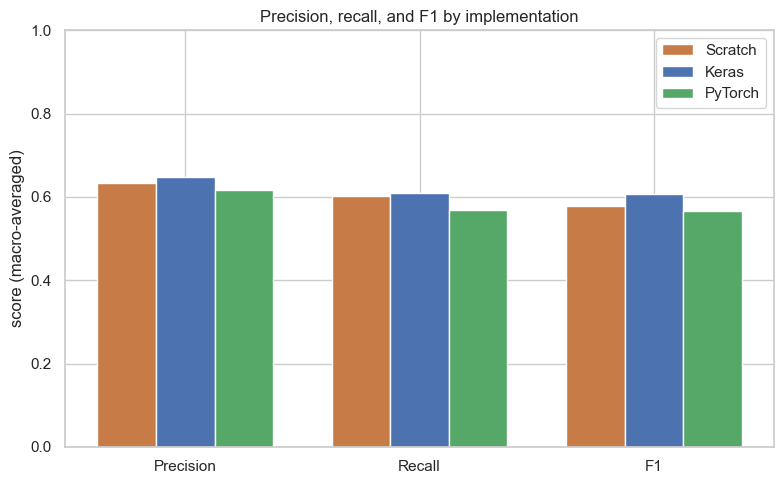
\includegraphics[width=0.7\linewidth]{images/cifar10_compare_prf1.png}
\caption{Precision, recall, and F1 (macro-averaged) by implementation.}
\end{figure}

\begin{figure}[H]
\centering
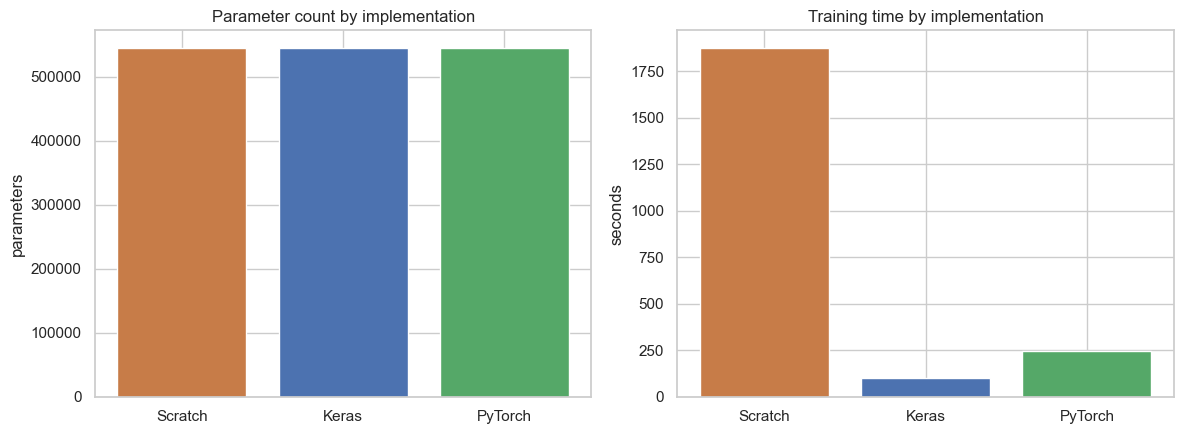
\includegraphics[width=\linewidth]{images/cifar10_compare_params_time.png}
\caption{Parameter count (identical across all three) and training time by
implementation. The scratch/framework training-time gap is the widest of the
three applications in this report.}
\end{figure}

\subsection{Comparison discussion}
\label{sec:cifar-compare}

Keras comes out slightly ahead on both accuracy (0.610) and F1 (0.608), with
scratch close behind (0.603 accuracy, 0.579 F1) and PyTorch trailing a little
further (0.570 accuracy, 0.566 F1). All three sit within about four points of
each other, the same order of spread seen for both other applications in this
report, consistent with three implementations of the same architecture rather
than three different models. The absolute accuracy here, in the low 60s, is
much lower than Fashion-MNIST's high 80s with the same architecture, and that
is expected: these are real color photographs compressed to $32\times32$
pixels, category pairs like cat/dog and automobile/truck are genuinely hard to
separate even at that resolution, and a two-convolution-layer network with no
data augmentation and only 12 epochs of plain SGD is a modest model for a
task at this level of difficulty. Accuracy in the low 60s here is not a sign
anything is broken; it is roughly what this architecture is capable of on
this data without the training tricks, augmentation, more epochs, a bigger
network, a fancier optimizer, deliberately left out to keep the three
implementations easy to compare against each other.

Training time repeats the pattern first seen in Fashion-MNIST, scratch is
dramatically slower than the other two, and the gap widens further here.
Scratch took 1,875.8 seconds (about 31 minutes) to train. Keras took 103.3
seconds. PyTorch took 244.1 seconds. Scratch was roughly 18.2 times slower
than Keras and 7.7 times slower than PyTorch, a wider multiple than
Fashion-MNIST's 17.6x/6.9x, despite this network having only modestly more
parameters (545,098 against 421,642). That points at input size and channel
count, three color channels instead of one, and a $32\times32$ image instead
of $28\times28$, rather than parameter count, as the real driver of scratch's
\code{im2col} convolution cost: both changes increase the amount of work the
first convolution's matrix multiply has to do, and scratch pays that cost
directly in wall-clock time with no framework-level optimization to absorb
it, while Keras's and PyTorch's compiled convolution operations scale far
more gracefully. Read together with Section \ref{sec:fm-compare}, a clean
three-point progression emerges across this report's three applications: the
diabetes MLP (Section \ref{sec:diabetes-compare}), scratch comparable in
speed to the frameworks, PyTorch actually slowest; the grayscale CNN, scratch
roughly 17.6x slower than Keras; the RGB CNN, scratch roughly 18.2x slower
than Keras. Training-time cost from building a network by hand grows
specifically with how much real convolution work the architecture asks for,
not with parameter count alone.

Which framework hid the most, and which gave the most control, is the same
answer as Fashion-MNIST's, for the same reasons: Keras hid the convolution,
the pooling, the backward pass, and the training loop behind one
\code{Sequential} definition and one \code{fit()} call; PyTorch hid only the
backward pass; scratch hid nothing. The three-application pattern across this
report is now clear: accuracy differences between scratch, Keras, and PyTorch
stay small, within a few points, whenever the architecture is genuinely held
fixed, the expected result and the main point of building the same network
three times. Training time differences, on the other hand, can be large and
depend heavily on what the architecture actually asks the hardware to do,
negligible for a tiny fully-connected network, large and specifically tied to
convolution workload for a CNN, a from-scratch NumPy implementation, however
correct, cannot match a mature framework's operator-level optimization for an
operation like convolution without adopting the same kind of low-level
optimization work those frameworks represent.

\newpage
% ---------------------------------------------------------------------
\section{Cross-Application Comparison}
\label{sec:cross}
% ---------------------------------------------------------------------

Table \ref{tab:cross-app} summarizes all three applications by test accuracy,
the primary metric used throughout this report since none of the three tasks
is regression, across all three implementations. Every cell is a
transposition of the per-application results tables in Sections
\ref{sec:diabetes}, \ref{sec:fashion}, and \ref{sec:cifar10}, not new
analysis.

\begin{table}[H]
\centering
\caption{Cross-application summary: test accuracy, all 3 applications x 3 implementations}
\label{tab:cross-app}
\begin{tabular}{llrr}
\toprule
Application & Implementation & Parameters & Accuracy \\
\midrule
\multirow{3}{*}{Diabetes}
  & Scratch & 2,177 & 0.7310 \\
  & Keras & 2,177 & 0.7533 \\
  & PyTorch & 2,177 & \textbf{0.7819} \\
\midrule
\multirow{3}{*}{Fashion-MNIST}
  & Scratch & 421,642 & \textbf{0.8973} \\
  & Keras & 421,642 & 0.8603 \\
  & PyTorch & 421,642 & 0.8660 \\
\midrule
\multirow{3}{*}{CIFAR-10}
  & Scratch & 545,098 & 0.6033 \\
  & Keras & 545,098 & \textbf{0.6102} \\
  & PyTorch & 545,098 & 0.5696 \\
\bottomrule
\end{tabular}
\end{table}

\noindent\textit{Bold marks the winning implementation in each application.
Parameter counts are identical across all three implementations within an
application, confirmed by a direct assertion in every notebook.}

\begin{table}[H]
\centering
\caption{Cross-application training time, seconds, all 3 applications x 3 implementations}
\label{tab:cross-time}
\begin{tabular}{lrrr}
\toprule
Application & Scratch & Keras & PyTorch \\
\midrule
Diabetes & 69.4 & \textbf{24.7} & 311.0 \\
Fashion-MNIST & 1,330.5 & \textbf{75.6} & 191.5 \\
CIFAR-10 & 1,875.8 & \textbf{103.3} & 244.1 \\
\bottomrule
\end{tabular}
\end{table}

\noindent\textit{Bold marks the fastest implementation in each application.
Keras is fastest in every application. Scratch is fastest of the two
non-Keras implementations only on diabetes, its tiny MLP; scratch is the
slowest implementation by a wide margin on both CNN applications.}

No single implementation wins every application, and the implementation that
wins by the widest margin, PyTorch on diabetes, is also the slowest
implementation on that same application, a direct illustration that accuracy
and training speed are independent axes here, not two views of the same
underlying quality.

% ---------------------------------------------------------------------
\section{Discussion}
\label{sec:discussion}
% ---------------------------------------------------------------------

\subsection{Did ``same architecture, different abstraction level'' actually hold?}

Yes, on the axis it makes the strongest claim about. Every application's
parameter count matched exactly across all three implementations, verified by
a direct assertion in each notebook rather than assumed, and every
application's accuracy spread across the three implementations stayed within
about four to five points, the kind of gap explainable by initialization
differences and the ordinary noise of training a fixed architecture rather
than evidence that one implementation is a fundamentally better learner.
Table \ref{tab:cross-app}'s flipping winner, PyTorch on diabetes, scratch on
Fashion-MNIST, Keras on CIFAR-10, is the pattern this claim predicts: if a
particular framework's implementation of "the same architecture" were
secretly a stronger model, it would win consistently, not take turns.

\subsection{Where the abstraction levels genuinely diverged}

Training time is where the three abstraction levels stopped behaving like
interchangeable views of the same computation. On the diabetes MLP, a tiny,
fully dense network, scratch and Keras trained in a comparable amount of
time, and PyTorch was actually the slowest implementation, its per-batch
autograd construction overhead a fixed cost too large for a 2,177-parameter
network's real computation to amortize away. Once real convolutions entered
the picture, Fashion-MNIST and CIFAR-10, that pattern reversed completely:
scratch became the slowest implementation by a wide and widening margin (17.6x
Keras on Fashion-MNIST, 18.2x Keras on CIFAR-10), because a from-scratch
\code{im2col} convolution, however correctly implemented and however much
faster than the naive position-loop it replaced, is still plain NumPy issued
from a Python training loop, with none of a mature framework's operator-level
optimization for convolution specifically. The gap widened again between the
two CNN applications in step with input size and channel count (CIFAR-10's
$32\times32\times3$ against Fashion-MNIST's $28\times28\times1$), not with
parameter count, which grew only modestly between the two (545,098 against
421,642). Visibility, correctness, and speed are three separate properties of
an implementation, and this project's own measured numbers show them trading
off in exactly the direction Lecture 04 predicts, more of the first two
costing real wall-clock time.

\subsection{What building every training loop by hand exposed}

Two findings surfaced specifically because this assignment kept scratch's
implementation fully visible rather than trusting a packaged \code{fit()}
call, and both are worth naming because a framework absorbs them silently.
First, the diabetes application's PyTorch loss value (Section
\ref{sec:diabetes-compare}) sits on a genuinely different numeric scale from
scratch's and Keras's, not because PyTorch trained a worse model, but because
\code{BCEWithLogitsLoss(pos\_weight=...)} reweights only the positive class's
loss term while scratch's manual weighting and Keras's \code{class\_weight}
both reweight every row. Three frameworks offering what looks like the same
named feature, balanced class weighting, actually parameterize it
differently underneath, exactly Lecture 04's own warning that different names
do not imply different concepts, read in reverse: sometimes the same name
does hide a real mechanical difference, and the only way to know is to check
the code, not trust the name. Second, the Fashion-MNIST scratch
implementation's own gradient-check cell caught a real bug during
development, a redundant $1/N$ division in the dense-layer backward pass
silently shrinking every dense-layer gradient, invisible from the outside
since the network still trained and still produced a plausible-looking loss
curve; only comparing the analytic gradient against a numerical
finite-difference approximation, layer by layer, surfaced it. Both findings
are the direct payoff of building the optimizer, the loss, and the gradient
computation by hand rather than importing them: a packaged implementation
would have absorbed either issue without ever surfacing it as something to
explain.

% ---------------------------------------------------------------------
\section{Conclusion}
% ---------------------------------------------------------------------

This report built three intelligent systems, diabetes risk screening (MLP),
Fashion-MNIST clothing recognition (CNN), and CIFAR-10 object recognition
(CNN), each with a single architecture implemented three separate times, from
scratch in NumPy with every forward pass, loss, backward pass, and parameter
update derived and coded by hand, in TensorFlow/Keras, and in PyTorch. Every
application's parameter count matched exactly across all three
implementations, and every application's accuracy spread stayed within a few
points, confirming Lecture 04's central claim that the conceptual architecture
is unchanged across abstraction levels, only its expression changes. What
genuinely differed, and differed by a large, measurable margin once real
convolutions were involved, was training time: a from-scratch NumPy
implementation, however correct, cannot match a mature framework's
operator-level optimization for an operation like convolution, a real cost of
full visibility that a tiny MLP's forward pass does not expose but a CNN's
does, and the gap widens further with input size and channel count rather
than with parameter count. Keeping every implementation's own training loop
and loss computation fully visible, rather than trusting a packaged
\code{fit()} call, is also what surfaced two concrete findings a framework
would have absorbed silently: PyTorch's \code{pos\_weight} class-weighting
mechanism scales the training loss differently from scratch's and Keras's
symmetric weighting despite sharing the same balanced-weighting intent, and a
redundant division bug in a from-scratch backward pass, caught only by a
numerical gradient check comparing hand-derived gradients against a
finite-difference approximation. Both are the kind of detail visible only to
someone who wrote every gradient by hand, exactly the payoff building a CNN
from scratch is meant to provide.

% ---------------------------------------------------------------------
\section{Reproducibility}
% ---------------------------------------------------------------------

\subsection{Environment}

\begingroup\sloppy\emergencystretch=3em
All three notebooks were built and executed in a dedicated virtual environment
at \texttt{assignment\_04/.venv} (Python 3.10.11, registered as Jupyter kernel
\texttt{assignment\_04}), with the following key package versions: numpy,
pandas, scikit-learn (metrics only), matplotlib, seaborn, jupyter, nbconvert,
nbformat, nbclient, tensorflow 2.21.0, torch 2.14.0+cpu, torchvision
0.29.0+cpu. CPU-only PyTorch/torchvision wheels were installed deliberately,
so the three-implementation training-time comparison is not confounded by one
implementation running on a different device class than the others.
\code{RANDOM\_SEED = 42} is fixed in every notebook for every split, shuffle,
and weight initialization (\code{np.random.seed}, Python's own
\code{random.seed}, \code{tf.random.set\_seed}, and
\code{torch.manual\_seed}, all set together).
\par\endgroup

\subsection{Re-running a notebook end to end}

Each application's notebook is self-contained and can be re-executed from its
own directory with:
\begin{footnotesize}
\begin{verbatim}
../.venv/Scripts/python.exe -m jupyter nbconvert \
    --to notebook --execute --inplace \
    notebook/<app>.ipynb --ExecutePreprocessor.timeout=1800
\end{verbatim}
\end{footnotesize}
replacing \texttt{<app>} with \texttt{diabetes}, \texttt{fashion\_mnist}, or
\texttt{cifar10}. Fashion-MNIST and CIFAR-10 download their datasets
automatically via \code{keras.datasets} on first run, no manual Kaggle step
required, unlike the diabetes application's CSV files, which must already be
present in \texttt{diabetes/data/}. Each notebook ends by saving all three
trained artifacts to its own \texttt{model/} directory:
\begin{itemize}[nosep]
  \item \texttt{scratch\_weights.npz}: the from-scratch implementation's
    trained parameters.
  \item \texttt{keras\_model.keras}: the trained Keras model.
  \item \texttt{pytorch\_model.pt}: the trained PyTorch model's state dict.
  \item \texttt{feature\_names.joblib} (diabetes only): the post-encoding
    feature column order.
  \item \texttt{input\_schema.json}: documented input fields and target.
\end{itemize}
followed by a reload-and-verify cell that reloads all three artifacts and
confirms their predictions match the in-memory versions computed during that
same run. No API, web, or mobile layer is included in this assignment, so no
additional run commands beyond notebook execution are required.

\end{document}
